\documentclass[bachelor,german]{hgbthesis}
\usepackage{xcolor}
\usepackage{listings}
\usepackage[utf8]{inputenc}
\usepackage{cmbright}
\usepackage[T1]{fontenc}
\usepackage{babel}
\definecolor{bluekeywords}{rgb}{0,0,1}
\definecolor{greencomments}{rgb}{0,0.5,0}
\definecolor{redstrings}{rgb}{0.64,0.08,0.08}
\definecolor{xmlcomments}{rgb}{0.5,0.5,0.5}

\lstdefinestyle{Java} { language=Java}
\lstdefinestyle{[Sharp]C} {language=[Sharp]C}

\lstset{language=[Sharp]C,
	captionpos=b,
	showspaces=false,
	showtabs=false,
	breaklines=true,
	showstringspaces=false,
	breakatwhitespace=true,
	escapeinside={(*@}{@*)},
	commentstyle=\color{greencomments},
	morekeywords={partial, var, value, get, set},
	keywordstyle=\color{bluekeywords},
	stringstyle=\color{redstrings},
	basicstyle=\ttfamily\small
}

\lstset{language=Java,
	captionpos=b,
  showspaces=false,
  showtabs=false,
  breaklines=true,
  showstringspaces=false,
  breakatwhitespace=true,
  commentstyle=\color{greencomments},
  keywordstyle=\color{bluekeywords},
  stringstyle=\color{redstrings},
  basicstyle=\ttfamily\small
}
\RequirePackage[utf8]{inputenc}		
\graphicspath{{images/}}    
\logofile{logo}						
\bibliography{literatur}  
\begin{document}
\title{Probleme in der Softwareentwicklung und wie Clean Code Development dabei unterstützen kann diese zu lösen}
\author{Stefan Kert}
\studiengang{Software Engneering}
\studienort{Hagenberg}
\abgabedatum{2016}{07}{14}	
\nummer{S1310307019} 
\betreuer{Josef ~Pichler, Dr.} 
\frontmatter
\maketitle
\tableofcontents

\chapter{Vorwort} 	% engl. Preface




		% ggfs. weglassen

\chapter{Kurzfassung}

An dieser Stelle steht eine Zusammenfassung der Arbeit, Umfang
max.\ 1 Seite. Im Unterschied zu anderen Kapiteln ist die
Kurzfassung (und das Abstract) üblicherweise nicht in Abschnitte
und Unterabschnitte gegliedert. 
Auch Fußnoten sind hier falsch am Platz.

Kurzfassungen werden übrigens häufig -- zusammen mit Autor und Titel
der Arbeit -- %
in Literaturdatenbanken aufgenommen. Es ist daher darauf zu
achten, dass die Information in der Kurzfassung für sich 
\emph{allein} (\dah ohne weitere Teile der Arbeit) zusammenhängend und
abgeschlossen ist. Insbesondere werden an dieser Stelle (wie \ua
auch im \emph{Titel} der Arbeit und im \emph{Abstract})
normalerweise \emph{keine Literaturverweise} verwendet! Falls
unbedingt solche benötigt werden -- etwa weil die Arbeit eine
Weiterentwicklung einer bestimmten, früheren Arbeit darstellt --,
dann sind \emph{vollständige} Quellenangaben in der Kurzfassung
selbst notwendig, \zB %
[\textsc{Zobel} J.: \textit{Writing for Computer Science -- The Art of
Effective Commu\-nica\-tion}. Springer-Verlag, Singa\-pur, 1997].

Weiters sollte daran gedacht werden, dass bei der Aufnahme in Datenbanken
Sonderzeichen oder etwa Aufzählungen mit "`Knödellisten"' in der
Regel verloren gehen. Dasselbe gilt natürlich auch für das 
\emph{Abstract}.


Inhaltlich sollte die Kurzfassung \emph{keine} Auflistung der
einzelnen Kapitel sein (dafür ist das Einleitungskapitel
vorgesehen), sondern dem Leser einen kompakten, inhaltlichen
Überblick über die gesamte Arbeit verschaffen. Der hier verwendete
Aufbau ist daher zwangsläufig anders als der in der Einleitung.
		
\chapter{Abstract}

\begin{english} %switch to English language rules
This should be a 1-page (maximum) summary of your work in English.
%und hier geht dann das Abstract weiter...
\end{english}

Im englischen Abstract sollte inhaltlich das Gleiche
stehen wie in der deutschen Kurzfassung. Versuchen Sie daher, die
Kurzfassung prä\-zise umzusetzen, ohne aber dabei Wort für Wort zu
übersetzen. Beachten Sie bei der Übersetzung, dass gewisse
Redewendungen aus dem Deutschen im Englischen kein Pendant haben
oder völlig anders formuliert werden müssen und dass die
Satzstellung im Englischen sich (bekanntlich) vom Deutschen stark
unterscheidet (mehr dazu in Abschn.\ \ref{sec:englisch}). Es
empfiehlt sich übrigens -- auch bei höchstem Vertrauen in die
persönlichen Englischkenntnisse -- eine kundige Person für das
"`proof reading"' zu engagieren.

Die richtige Übersetzung für "`Diplomarbeit"' ist übrigens
schlicht \emph{thesis}, allenfalls  "`diploma thesis"' oder "`Master's thesis"', 
auf keinen Fall aber "`diploma work"' oder gar "`dissertation"'. 
Für "`Bachelorarbeit"' ist wohl "`Bachelor thesis"' die passende Übersetzung. 

Übrigens sollte für diesen Abschnitt die \emph{Spracheinstellung} in \latex\ von Deutsch
auf Englisch umgeschaltet werden, um die richtige Form der
Silbentrennung zu erhalten, die richtigen Anführungszeichen müssen allerdings selbst gesetzt werden %
(s.\ dazu die Abschnitte \ref{sec:sprachumschaltung} %
und \ref{sec:anfuehrungszeichen}).
			

\mainmatter 

\chapter{Einleitung}
\label{cha:Einleitung}

\section{Problemstellung}
Eine sehr zentrale Eigenschaft von Software ist die Tatsache, dass immer wieder Änderungen stattfinden. Durch die Entwicklung, welche meist über lange Zeit von verschiedenen Programmierern oder Programmiererinnen vorgenommen wird, ergibt sich meist ein sehr unlesbarer, schwer zu wartender und schwer zu testender Code.
Diese Probleme führen in weitere Folge zu Qualitätseinbußen, da durch die schlechte Testbarkeit schlichtweg auf wichtige Tests verzichtet wird, da die Zeit für
die Implementierung dieser zu lange dauern würde. Eine weitere Folge der schlechten Lesbarkeit, ist die sich daraus ergebenden Schwierigkeiten beim Ändern des vorhandenen Codes. Dieser lässt sich nämlich nur noch unter sehr großem Aufwand und sehr großem Risiko, da er meist auch nicht durch Tests abgedeckt ist ändern,
was wiederum dazu führt, dass weniger Änderungen vorgenommen werden. Im schlimmsten Fall führen diese Probleme schlussendlich zum Scheitern des Projektes und es 
muss eingestellt werden, da der Aufwand der nötig wäre neue Änderungen oder Fehlerbehebungen vorzunehmen zu groß wäre. 

\section{Motivation}
In der modernen Softwareentwicklung geht es in erster Linie um das Umsetzen funktionaler sowie nicht funktionaler
Anforderungen und um die Behebung von Fehlern welche bei der Umsetzung dieser Anforderungen häufig auftreten. Ein wichtiger Punkt dabei ist, den Code so zu gestalten, dass er nicht nur vom Programmierer, der ihn geschrieben hat, gelesen werden kann, sondern auch von anderen Programmieren und dies auch möglichst noch nach mehreren Monaten. Um dies zu erreichen, müssen gewisse Grundsätze angewendet werden. In den letzten Jahren hat sich zu diesem Thema eine Strömung ergeben welche sich als Clean Code Development (im folgenden nur noch als CCD abgekürzt) bezeichnet. Geprägt wurde diese Bewegung in erster Linie von Robert. C. Martin und seinem Bestseller Clean Coder. Umso genauer man darauf achtet, den Code beim Schreiben lesbar zu gestalten, umso leichter wird es diesen auch noch nach einiger Zeit wieder zu Lesen. Bei schlecht geschrieben Code kann es sein, dass man bereits nach einigen Tagen nicht mehr genau weiß, was man damit bezwecken wollte. 

\section{Lösungsvorschlag}
CCD bietet für diese Probleme eine Lösung, welche aber über mehrere Jahre hinweg in den Entwicklungsteams etabliert werden muss. Der wichtigsten Punkte in CCD sind die folgenden:

\begin{figure}[h]
	\centering
		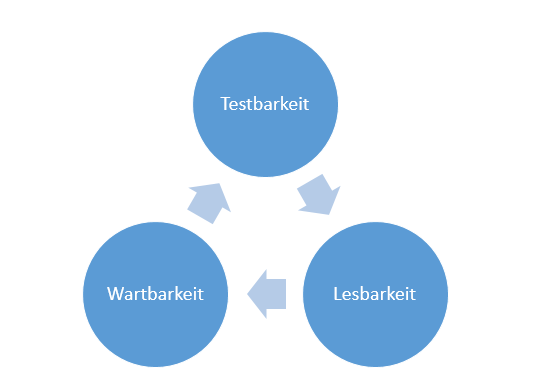
\includegraphics[width=1.00\textwidth]{images/cycle.PNG}
	\caption{CCD Zyklus}
	\label{fig:cycle}
\end{figure}

In der Abbildung \ref{fig:cycle} kann man gut erkennen, dass diese drei Hauptpunkte voneinander abhängen. Durch die gute Lesbarkeit, wird die Wartbarkeit des Codes erhöht da sich selbst ein neuer Mitarbeiter schnell einlesen kann und gut erkennen kann welche Aufgabe der aktuell betrachtete Code hat. Durch die bessere Wartbarkeit ergibt sich im weiteren auch die besseren Testbarkeit, welche für die Qualität der Software von hoher Bedeutung ist, da nur für getesteten Code sichergestellt werden kann, dass dieser auch wirklich die gewünschte Aufgabe richtig erledigt. Diese verbesserte Testbarkeit führt schließlich zu einer besseren Lesbarkeit, da die Test mit einer Dokumentation des Codes verglichen werden können. Sie zeigen welche Ausgabe erwartet werden kann und meist zeigen diese Tests auch Grenzfälle.


\chapter{Clean Code Development Grundlagen}
\section{Womit beschäftigt sich CCD?}
\SuperPar Wie in der Einleitung bereits erläutert beschäftigt sich CCD in erster Linie mit dem Schreiben von lesbaren Code. Es sollte dabei bei der Implementierung geachtet werden, dass
In der Abbildung \ref{fig:cycle} ist ein Kreislauf dargestellt, der die drei Hauptpunkte darstellt und auch zeigt, dass diese sich gegenseitig beeinflussen. Durch die gute Lesbarkeit, wird die Wartbarkeit des Codes erhöht. Da sich selbst ein neuer Mitarbeiter schnell einlesen kann und gut erkennen kann welche Aufgabe der aktuell betrachtete Code hat sind die Einarbeitungszeiten für Mitarbeiter außerdem viel kürzer. Durch die bessere Wartbarkeit ergibt sich im weiteren auch die besseren Testbarkeit, welche für die Qualität der Software von hoher Bedeutung ist, da nur für getesteten Code sichergestellt werden kann, dass dieser auch wirklich die gewünschte Aufgabe richtig erledigt. Diese verbesserte Testbarkeit führt schließlich zu einer besseren Lesbarkeit, da die Test mit einer Dokumentation des Codes verglichen werden können. Sie zeigen welche Ausgabe erwartet werden kann und meist zeigen diese Tests auch Grenzfälle.

\begin{figure}[h]
	\centering
		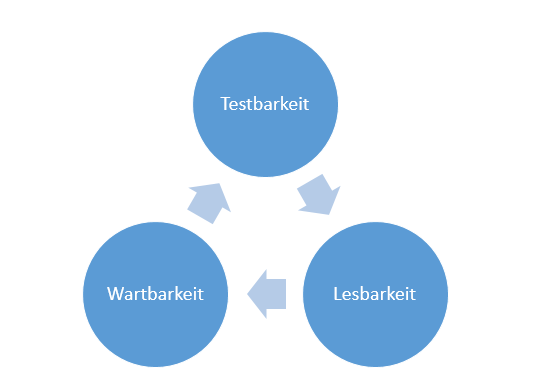
\includegraphics[width=1.00\textwidth]{images/cycle.PNG}
	\caption{CCD Zyklus}
	\label{fig:cycle}
\end{figure}

\section{Ziele von CCD}
\SuperPar Die wichtigsten Ziele von CCD sind es, den Quellcode 

\section{Die Pfadfinder-Regel}
\SuperPar Eine der grundlegendsten Regeln im CCD ist die sogenannte Pfadfinder-Regel. Robert C. Martin definiert diese in \cite{CleanCode} wie folgt:

\begin{quote}
	Hinterlasse den Campingplatz sauberer, als du ihn gefunden hast.
\end{quote}

\SuperPar Auf die Arbeit eines Programmierers oder einer Programmiererin umgemünzt bedeutet dieser Leitsatz, dass jede Klasse, welche man auscheckt oder betrachtet verbessert werden sollte. Dies muss nicht immer ein großes Refactoring oder ein verbessern der Gesamtstruktur sein. Es reicht meist schon, für eine Variable einen besseren Namen zu vergeben, oder einen unnötigen Kommentar zu entfernen. Robert C. Martin schreibt weiters, dass sich durch dieses vorgehen ein für die Softwareentwicklung ungewöhnlicher Trend ergibt. Der Quelltext wird über die Zeit besser. Er verbindet dieses Verhalten außerdem mit professionelem Verhalten. Ein professioneller, verantwortungsbewusster Programmierer versucht ständig, die Codebasis zu verbessern.

\section{Smells und Heuristiken}
\SuperPar Robert C. Martin beschreibt in \cite{CleanCode} eine Liste von Smells und Heuristken, welche Probleme beschreiben, die sehr häufige Ursachen für schlechten Code darstellen.
\subsection{Kommentare}

\begin{table}[h]
	\centering
		 \begin{tabular}{ | l | }
		 \hline
			Name \\  \hline
			Ungeeignete Informationen\\
			Überholte Kommentare  \\
			Redundante Kommentare \\
			Schlecht geschriebene Kommentare  \\
			Auskommentierter Code \\ \hline
		\end{tabular}
	\caption{Smells und Heuristiken für Kommentare}
	\label{tab:SmellsUndHeuristiken_Comments}
\end{table}

\subsection{Umgebung}

\begin{table}[h]
	\centering
		 \begin{tabular}{ | l | }
		 \hline
			Name \\  \hline
			Ein Build erfordert mehr als einen Schritt \\
			Test erfordern mehr als einen Schritt \\ \hline
		\end{tabular}
	\caption{Smells und Heuristiken für die Umgebung}
	\label{tab:SmellsUndHeuristiken_Umgebung}
\end{table}

\subsection{Funktionen}

\begin{table}[h]
	\centering
		 \begin{tabular}{ | l | }
		 \hline
			Name \\  \hline
			Zu viele Argumente \\
			Output-Argumente \\
			Flag-Argumente \\
			Tote Funktionen \\ \hline
		\end{tabular}
	\caption{Smells und Heuristiken für Funktionen}
	\label{tab:SmellsUndHeuristiken_Functions}
\end{table}

\subsection{Allgemein}

\begin{table}[h]
	\centering
		 \begin{tabular}{ | l | }
		 \hline
			Name \\  \hline
			Mehrere Sprachen in einer Quelldatei \\
			Offensichtliches Verhalten ist nicht implementiert \\
			Falsches Verhalten an den Grenzen \\
			Übergangene Sicherungen \\
			Duplizierung \\
			Auf der falschen Abstraktionsebene codieren \\
			Basisklasse hängt von abgeleiteten Klassen ab \\
			Zu viele Informationen \\
			Toter Code \\
			Vertikale Trennung \\
			Inkonsistenz \\
			Müll \\
			Künstliche Kopplung \\
			Funktionsneid \\
			Selektor-Argumente \\
			Verdeckte Absicht \\
			Falsche Zuständigkeit \\
			Fälschlich als statisch deklarierte Methode \\
			Aussagekräftige Variablen verwenden \\
			Funktionsname sollte die Aktion ausdrücken \\
			Den Algorithmus verstehen \\
			Logische Abhängikeiten in phyische umwandeln \\
			Polymorphismus statt If/Else oder Switch/Case verwenden \\
			Konventionen beachten \\
			Magische Zahlen durch benannte Konstanten ersetzen \\
			Präzise sein \\
			Struktur ist wichtiger als Konvention \\
			Bedingungen einkapseln \\
			Negative Bedingungen vermeiden \\
			Eine Aufgabe pro Funktion! \\
			Verborgene zeitliche Kopplungen \\
			Keine Willkür \\
			Grenzbedingungen einkapseln \\
			In Funktionen nur eine Abstraktionsebene tiefer gehen \\
			Konfigurierbare Daten hoch ansiedeln \\
			Transitive Navigation vermeiden \\ \hline
		\end{tabular}
	\caption{Smells und Heuristiken für Kommentare}
	\label{tab:SmellsUndHeuristiken_Comments}
\end{table}

\subsection{Namen}

\begin{table}[h]
	\centering
		 \begin{tabular}{ | l | }
		 \hline
			Name \\  \hline
			Deskriptive Namen wählen \\
			Namen sollten der Abstraktionsebene entsprechen \\
			Möglichst die Standardnomenklatur verwenden \\
			Eindeutige Namen \\
			Lange Namen für große Geltungsbereiche \\
			Codierungen vermeiden \\
			Namen sollten Nebeneffekte beschreiben \\ \hline
		\end{tabular}
	\caption{Smells und Heuristiken für die Umgebung}
	\label{tab:SmellsUndHeuristiken_Umgebung}
\end{table}


\subsection{Tests}

\begin{table}[h]
	\centering
		 \begin{tabular}{ | l | }
		 \hline
			Name \\  \hline
			Unzureichende Tests \\
			Ein Coverage-Tool verwenden \\
			Triviale Tests nicht überspringen \\
			Ein ignorierter Test zeigt eine Mehrdeutigkeit auf \\
			Grenzbedingungen testen \\
			Bei Bugs die Nachbarschaft gründlich testen \\
			Das Muster des Scheiterns zur Diagnose nutzen \\
			Hinweise druch Coverage-Patterns \\
			Testen sollten schnell sein \\ \hline
		\end{tabular}
	\caption{Smells und Heuristiken für die Umgebung}
	\label{tab:SmellsUndHeuristiken_Umgebung}
\end{table}

\section{Coding Conventions}
\label{cha:CodingConventions}
Coding Conventions sind ein sehr effizientes Mittel projektweite, oder auch unternehmensweite Regeln zu definieren, wie einzelne Aspekte der Programmierung gestaltet werden sollten. Vor allem für Opensource Projekte ist dies ein sehr wichtiges Mittel wie ein durchgängiger Codierungsstil gewählt werden kann. Meist werden auch für Frameworks Coding Conventions definiert wie zum Beispiel für C\# \cite{CSHARPCoding}. Meist werden diese grundlegenden Konventionen von Unternehmen verwendet und nur teilweise angepasst, da es durch einen durchgängigen Programmierstil für eine Plattform leichter ist, dass sich neue Programmierer oder Programmiererinnen in die Codebasis einarbeiten. Ein wichtiger Aspekt der bei Coding Conventions beachtet werden muss, ist die Möglichkeit der automatischen Überprüfung dieser. Dazu werden in Abschnitt \ref{cha:CheckingCCDCriterias} einige Möglichkeiten erläutert, wie die Überprüfung dieser Kriterien erfolgen kann.

 
\section{Überprüfung der CCD Kriterien}
\label{cha:CheckingCCDCriterias}
\SuperPar Häufig stellt sich beim CCD die Frage, wie es möglich ist die einzelnen Kriterien zu überprüfen. Hierzu gibt es verschiedene Varianten. Es gibt einerseits die statische Codeanalyse, welche dafür Sorgen kann, dass die in Abschnitt \ref{cha:CodingConventions} beschriebenen Coding Conventions eingehalten werden. Ein sehr wirksames Mittel für die Überprüfung des Quellcodes allgemein sind Coding Reviews. Es sollte in den folgenden Abschnitten näher auf diese beiden Werkzeuge eingegangen werden.

\subsection{Statische Codeanalyse}
\SuperPar Die statische Codeanalyse bietet eine Möglichkeit zur Analyse des Quellcodes nach fix vorgegebenen Regeln. Dabei werden für ein Unternehmen, oder für ein Projekt die Abschnitt \ref{cha:CodingConventions} beschriebenen Coding Conventions festegelegt und an Hand dieser Regeln definiert. Ein Beispiel für solch eine Regel wäre das in C\# übliche \textit{I} vor einem Interfacenamen. Das Tool für die statische Codeanalyse würde im Falle einer Missachtung dieser Regel eine Warnung ausgeben und der Programmierer würde direkt darauf aufmerksam gemacht werden, dass er sich nicht an die Coding Conventions hält. Im .NET Bereich ist das wohl bekannteste statische Codeanalyse Tool NDepend (http://www.ndepend.com/). Mit diesem ist es neben den überprüfen der Coding Conventions auch möglich, zirkuläre Abhängigkeiten zwischen Klassen zu erkennen, zyklische Komplexitäten von Methoden zu analysieren und viele weitere Metriken zu erzeugen, die Aufschluss darüber geben, wie sauber der analysierte Code programmiert wurde. Im Java Bereich gibt es das sehr hilfreiche Tool JDepend (http://clarkware.com/software/JDepend.html) welches ähnlich aufgebaut ist wie NDepend.

\subsection{Code Reviews}
\SuperPar Code Reviews sind ein sehr wirksames Mittel um geschriebenen Code zu Überprüfen. Es handelt sich bei diesen Reviews um manuelle Überprüfungen, die meist von erfahreneren Entwicklern vorgenommen werden. Dabei ist einer der wichtigsten Punkte, dass das Review nicht durch die Person erfolgt, die den Quellcode produziert hat, sondern durch jemand anderen. Weiters gibt es die Möglichkeit ein sogenanntes Peer Review durchzuführen. Bei diesem führen die Person, die den Quellcode produziert hat und eine zweite Person das Review durch und besprechen den vorliegenden Code. An dieser Stelle sollte das Prinzip des Pair Programmings, das aus dem Extreme Programming kommt erwähnt werden. \cite{BeckExtreme} 
\chapter{Analyse verschiedener Problemstellungen in der Softwareentwicklung}

\SuperPar In diesem Abschnitt erfolgt die Analyse einiger wichtiger CCD Kriterien, welche im Buch Clean Code von Robert C. Martin beschriebenen sind. Dabei dienen verschiedene Opensource Frameworks zur Veranschaulichung dieser. Die einzelnen Kriterien, welche zur Analyse ausgewählt wurden, sind einige der am häufigsten missachteten Regeln und diese werden daher genauer betrachtet.

\SuperPar Folgende Frameworks dienen der Veranschaulichung:

\begin{itemize}
	\item Log4net (.NET)
	\item Hibernate (Java)
	\item Roslyn (.NET)
	\item Swift (C++)
\end{itemize}
\newpage
\section{Duplizierungen beim Entwickeln von Software}
\SuperPar Eines der größten Probleme bei der Entwicklung von Software stellt die Duplizierung dar. Dabei lässt sich Duplizierung nicht nur im Code finden, sondern auch in anderen Vorgängen die für die Softwareentwicklung von Bedeutung sind. Für jeden Entwickler gibt es zahlreiche Aufgaben, welche er immer wieder erledigen muss. Diese sollten möglichst automatisiert und mit wenig Aufwand möglich sein, da dies ansonsten eine Duplizierung der Arbeit bedeuten würde.

\SuperPar Auf Code bezogen verbirgt sich Duplizierung nicht immer nur auf Bibliothek-, oder Klassenebene, sondern auch in Methoden. Dabei muss man zwischen einfacher, und logischer Duplizierung unterscheiden. Bei der einfachen Duplizierung handelt es sich um schlichtweg gleichen Code. Meist wurde dieser kopiert und nur ein wenig angepasst. Die logische Duplizierung ist meist schwieriger zu erkennen, denn in diesem Fall sind die duplizierten Stellen vom Aufbau her unterschiedlich, sie gleichen sich aber in der Aufgabe welche diese erledigen. Oft treten solche logischen Duplizierungen, wenn bei der Benennung der vorhandenen Methoden beziehungsweise Klassen nicht auf eine ausreichend offensichtliche Namensgebung geachtet wurde. Ein sehr wichtiges Prinzip hinsichtlich Codeduplizierung ist das von Dave Thomas und Andy Hunt beschrieben DRY-Prinzip (Don´t Repeat Yourself \cite{PRAG1999}).

\SuperPar Wie bereits erwähnt, ergeben sich durch die Duplizierung zahlreiche Probleme. Einerseits müssen Arbeiten doppelt erledigt werden, andererseits kann im Falle eines Fehlers auf das Beheben dieses in einem duplizierten Abschnitt vergessen werden.

\SuperPar Robert C. Martin bietet in seinem Buch Clean Code einige Möglichkeiten wodurch diese Probleme vermieden werden können. Diese sollten im folgenden Abschnitt näher betrachtet werden.

\subsection{Duplizierung boolscher Ausdrücke}
\label{cha:BadBoolStatements}
\begin{itemize}
	\item Projekt: \textit{Hibernate}
	\item Programmiersprache: \textit{Java}
	\item Betreffende Klasse: \textit{AbstractPropertyHolder}
	\item Betreffendes Paket: \textit{org.hibernate.cfg}
\end{itemize}

\SuperPar Wie bereits erwähnt, treten Codeduplizierungen nicht nur auf Bibliothek-, bzw. Klassenebene auf, sonder meist in einem viel kleineren Kontext. Bei boolschen Ausdrücken ist dies sehr oft der Fall. Eine logische Verzweigung, welche auf zum Beispiel die Validität einer Eingabe prüft, könnte Dies ist oft ein sehr subtiles Problem und kann nicht so leicht festgestellt werden. Meist ist dies bei komplexen boolschen Ausdrücken der Fall. Diese werden oft von mehreren Funktionen benötigt und daher einfach in den einzelnen Funktionen verwendet. Ein Beispiel für so einen boolschen Ausdruck befindet sich in Listing \ref{BoolStatement1}.

\begin{lstlisting}[language=Java, caption=Komplexe boolsche Ausdrücke 1 Zeile 255 - 264, label=lst:BoolStatement1]
	@Override
	public JoinColumn[] getOverriddenJoinColumn(String propertyName) {
		JoinColumn[] result = getExactOverriddenJoinColumn( propertyName );
		if ( result == null && propertyName.contains( ".collection&&element." ) ) {
			//support for non map collections where no prefix is needed
			//TODO cache the underlying regexp
			result = getExactOverriddenJoinColumn( propertyName.replace( ".collection&&element.", "."  ) );
		}
		return result;
	}
\end{lstlisting}

\SuperPar Ein paar Zeilen weiter in derselben Klasse findet sich die in Listing \ref{lst:BoolStatement2} dargestellte Methode.

\begin{lstlisting}[language=Java, caption=Komplexe boolsche Ausdrücke 2 Zeile 305 - 313, label=lst:BoolStatement2]
public JoinTable getOverriddenJoinTable(String propertyName) {
	JoinTable result = getExactOverriddenJoinTable(propertyName);
	if(result == null 
		&& propertyName.contains(".collection&&element.")){
		//support for non map collections where no prefix is needed
		//TODO cache the underlying regexp
		result = getExactOverriddenJoinTable( propertyName.replace( ".collection&&element.", "."  ) );
	}
	return result;
}
\end{lstlisting}

\SuperPar Konkret geht es in diesem Beispiel um den in Listing \ref{lst:BoolStatement3} beschriebenen boolschen Ausdruck der in dieser Klasse insgesamt drei mal vorkommt.

\begin{lstlisting}[language=Java, caption=Boolscher Audruck, label=lst:BoolStatement3]
result == null && propertyName.contains(".collection&&element.")
\end{lstlisting}

\SuperPar Wie man anhand dieser Listings leicht erkennen kann, wird dieser Ausdruck in beiden Methoden verwendet, wodurch sich eine Code Duplizierung ergibt. Dieses Problem kommt vor allem bei zukünftigen Änderungen zu Tragen. Wenn zum Beispiel für die Variable \textit{propertyName} eine \textit{XML-Zeichenkette} übergeben wird und die Überprüfung wie in Listing \ref{lst:OtherSyntaxForBool} dargestellt erfolgen müsste, würde dies eine Änderung in allen Funktionen welche dieses boolsche Statement verwenden nach sich ziehen. 

\begin{lstlisting}[language=Java, caption=Boolscher Ausdruck neu, label=lst:BoolStatement4]
 propertyName.contains("</collectionType><element>")
\end{lstlisting}

\SuperPar Falls beim Ändern der Überprüfung auf eine der Funktionen, in denen diese verwendet wird, vergessen wird, würde dies zu einem Fehler führen. Ein weiteres Problem, das sich hier wie bereits oben beschrieben ergibt, ist die Tatsache, dass dieser boolsche Kommentar ohne einen Kommentar oder ein genaues Lesen sehr schwer zu verstehen ist. Man könnte hier beide Probleme beseitigen, in dem man aus dem boolschen Audruck eine eigene Methode extrahiert. Dabei wird hier nur der zweite Teil des boolschen Ausdrucks extrahiert, da der erste Teil mit dem Nullcheck spezifisch für die einzelnen Methoden verwendet werden muss. Eine solche Methode könnte wie in Listing \ref{BoolStatement4} aussehen.

\begin{lstlisting}[language=Java, caption=Boolscher Ausdruck neu, label=lst:BoolStatement4]
private bool isPlaceholderForCollectionAndElementInPropertyName(String propertyName) {
	return propertyName.contains(".collection&&element.");
}
\end{lstlisting}

Durch ein Extrahieren der Überprüfung des Parameters \textit{propertyName} kann für diese Methode ein eigener Name gewählt werden, der klar den Zweck dieser Überprüfung vermittelt und durch diese Extrahierung wird auch die sehr problematische Codeduplizierung verhindert. Codeduplizierungen eliminiert und es bleibt nur noch die Sicherheitsüberprüfung auf null.

\subsection{Testen, Erzeugen und Verteilen von Software}

\SuperPar In der modernen Softwareentwicklung spricht man oft von \textit{Continous Delivery}. Dabei geht es um die azyklische Auslieferung von Software. Es wird dabei eine Pipeline eingerichtet, welche die einzelnen Aufgaben, welche für die Auslieferung von Software nötig sind ausführt. In dem Buch \textit{Continuous Delivery} von Eberhard Wolff erläutert der Autor seine Gedanken zum automatisieren des Prozesses vom Erstellen der Software, über das Testen bis zur Auslieferung dieser. Dies sollte für das Team möglichst einfach möglich sein und einmalig eingerichtet, für jeden zugänglich sein, sodass man möglichst schnell eine Rückmeldung erhält, ob die aktuellen Änderungen Probleme verursacht haben. Dies sollte für das Team über eine sogenannte \textit{Continous Integration} Komponente möglich sein.

\SuperPar Der automatische Prozess des Erzeugens und des Testens sollte jedoch nicht nur über die \textit{Continous Integration} Komponente ermöglicht werden. Es sollte für jeden Programmierer durch wenige Schritte möglich sein, die Software zu Erzeugen und die Tests auch auszuführen. Dies sollte möglichst durch einen einzigen Befehl, durch einen einzigen Klick, oder wenn möglich sogar automatisiert erledigt werden. Es sollten dafür keine komplizierten Operationen nötig sein, da dies zu einer Duplizierung der Arbeit führt und immer wieder Zeit benötigt. Mit modernen Entwicklungsumgebungen wie Visual Studio oder Eclipse sind meist schon Werkzeuge integriert, welche das Erstellen und das Testen von Software durch eine einfache Tastenkombination oder einen einzelnen Klick ermöglichen. Diese Features sollten daher auch verwendet werden.

\subsection{Redundante Kommentare}
\begin{itemize}
	\item Projekt: \textit{Log4Net}
	\item Programmiersprache: \textit{C\#}
	\item Betreffende Klasse: \textit{ConfigurationChangedEventArgs}
	\item Betreffender Namespace: \textit{log4net.Repository}
\end{itemize}

\SuperPar Redundante Kommentare findet man sehr häufig in den verschiedensten Projekten. Oft werden für Methoden Kommentare geschrieben, welche nicht mehr als den Namen der Methode beinhalten. Dies führt natürlich zu keiner Verbesserung der Lesbarkeit und führt im Weiteren auch zu einer Aufblähung des Codes. Sehr häufig tritt dieses Problem auch bei Vorgeschriebenen Kommentaren auf. bei denen es in Coding Conventions vorgeschrieben ist, dass jede Methode einen Header zur Dokumentation
bekommen sollte. Dabei kommt es häufig zu redundanten Kommentaren, welche keinen wirklichen Mehrwert bringen. Robert C. Martin schreibt hierzu (Clean Code, Seite 93 - 96), dass solche Regeln meist zu Verwirrung, Lügen und einer allgemeinen Unordnung führen. 

\SuperPar Wenn man nun das in Listing \ref{lst:RedundantComment} stehende Beispiel betrachtet, fällt einen sofort der Kommentar auf, welcher keine richtigen Mehrwert
für den Leser bringt. Wie Robert C. Martin erwähnt, führt dieser nur zu einer Unordnung und kann im schlimmsten Fall sogar zu einer fälschlichen Information führen,
falls der Parameter umbenannt wird und der Kommentar dafür nicht angepasst wird. Auf Grund dieser Tatsache, sollte man laut Robert C. Martin auch auf solche Regeln verzichten, da diese eben genau zu den genannten Probleme führen.

\begin{lstlisting}[language={[Sharp]C}, caption=Beispiele für überflüssige Kommentare, label=lst:RedundantComment]
/// <summary>
/// 
/// </summary>
/// <param name="configurationMessages"></param>
public ConfigurationChangedEventArgs(ICollection configurationMessages)
{
		this.configurationMessages = configurationMessages;
}
\end{lstlisting}

\section{Komplexe Strukturen und schwer zu verstehende Konstrukte}

\SuperPar Sehr oft kommt es in der Softwareentwicklung zu einer sehr komplexen Struktur der einzelnen Komponenten. Klassen mit sehr vielen Funktionen. Funktionen, welche mehr als eine Aufgabe erfüllen und daher oft sehr lange werden. Nicht mehr benötigte Codeabschnitte, welche aus Angst vor einem Verlust dieser nicht gelöscht werden. Dies sind nur einige der Probleme, welche in der Softwareentwicklung auftreten können. Viele dieser Probleme sind leicht zu lösen. Durch moderne Versionsverwaltungssysteme ist es nicht mehr nötig Codeabschnitte, die nicht mehr benötigt werden auszukommentieren. Diese können einfach gelöscht werden. Einige Probleme, welche sich zum Beispiel bei Klassen mit sehr vielen Methoden ergeben, können nur durch Erfahrung und Übung erkannt werden. Es sollte bei Klassen und Funktionen vor allem darauf geachtet werden, dass diese nur genau einen Zweck erfüllen. Ein weiterer wichtiger Indikator, ob eine Komponente gut programmiert ist, ist die Testbarkeit dieser. Bei schlecht programmierten beziehungsweise geplante Klassen ist es nur sehr schwer - oder gar nicht - möglich diese zu Testen. Im folgenden Abschnitt werden die häufigsten Probleme für komplexe Strukturen beziehungsweise schwer zu verstehende Konstrukte aufgearbeitet.

\subsection{Auskommentierter Code}
\begin{itemize}
	\item Projekt: \textit{Hibernate}
	\item Programmiersprache: \textit{Java}
	\item Betreffende Klasse: \textit{BindHelper}
	\item Betreffendes Paket: \textit{org.hibernate.cfg}
\end{itemize}


\SuperPar Code der nicht mehr benötigt wird, wird häufig einfach auskommentiert und bleibt danach über lange Zeit im Quellcode bestehen. Dies wäre jedoch bei den modernen Versionsverwaltungssystemen gar nicht mehr notwendig, da diese eine genaue Auflistung der gelöschten, geänderten oder hinzugefügten Abschnitte anbieten. Es ist mit diesen auch leicht möglich Abschnitte, die man gelöscht hat, wieder aufzufinden, sowie diese wiederherzustellen. Code der nicht mehr benötigt wird sollte daher einfach gelöscht werden und mit einer vernünftigen Commit Message versehen werden. Im Hibernate Framework ist eine Klasse die einen solchen auskommentierten Codeabschnitt enthält die \textit{BindHelper} Klasse. Eine sehr problematische Stelle befindet sich in dieser Klasse in Zeile 421. Dort gibt es den in Listing \ref{lst:CommentedCode} beschriebenen Codeabschnitt.

\begin{lstlisting}[language=Java, caption=Beispiele für auskommentierten Code, label=lst:CommentedCode]
/*FIXME cannot use subproperties becasue the caller needs top level properties
//if (property.isComposite()) {
//	Iterator subProperties = ((Component)property.getValue()).getPropertyIterator();
// 	while (subProperties.hasNext()) {
//  	matchColumnsByProperty(((Property)subProperties.next()), columnsToProperty);
// 	}
}*/ 
\end{lstlisting}

\SuperPar Der Kommentar deutet darauf hin, dass es in diesem Codeabschnitt einen Fehler gibt der behoben werden müsste. Anstatt diesen Fehler zu beheben wurde der Code einfach auskommentiert und nach einigen Wochen weiß niemand mehr, dass es diesen Fehler gibt. Hier sollte entweder in einem Issue Tracking System genau mitdokumentiert werden, wo der Fehler auftritt und Möglichkeiten diesen zu beheben, oder den Fehler direkt zu beheben. Diesen einfach stehen zu lassen und die fehlerhafte Codestelle auszukommentieren ist dabei wohl der schlechteste Weg, da so der Fehler nicht mehr auftreten wird und er somit vergessen wird, wodurch sich vermutlich weitere Probleme ergeben. Auch Robert C. Martin schlägt in seinem Buch eine sehr pragmatische Lösung vor: Auskommentierter Code sollte immer gelöscht werden, da er zusätzlich zu den genannten Gründen auch den Quellcode unnötig aufbläht.

\subsection{Kapseln von Errorhandling in eigene Methoden}
\begin{itemize}
	\item Projekt: \textit{Roslyn}
	\item Programmiersprache: \textit{C\#}
	\item Betreffende Klasse: \textit{MetadataAndSymbolCache}, \textit{FileKey}
	\item Betreffender Namespace: \textit{Microsoft.CodeAnalysis.CompilerServer}, \textit{Roslyn.Utilities}
\end{itemize}

\SuperPar Das behandeln von Fehlern und Ausnahmen ist ein sehr zentraler Aspekt eines jeden Programmes. Eine richige und gut implementierte Strategie zur Fehlerbehandlung kann sehr viel Einfluss auf die Wartbarkeit eines Programmes haben. Oft wird dabei Logik und Fehlerbehandlung vermischt, was meist zu einer Verschlechterung der Lesbarkeit führt. Da es bei der Fehlerbehandlung um einen eigenen Aspekt geht, sollte diese in eine eigene Methode ausgelagert werden. Diese Methode ist dabei ein Wrapper für die zu behandelte Methode. Ein Beispiel aus dem Quelltext von Roslyn ist die in Listing \ref{lst:AspectedErrorhandling1} gezeigte Methode.

\begin{lstlisting}[language={[Sharp]C}, caption=Beispiele für getrennten Aspket der Fehlerbehandlung, label=lst:AspectedErrorhandling1]
private FileKey? GetUniqueFileKey(string filePath)
{
	try
	{
		return FileKey.Create(filePath);
	}
	catch (Exception)
	{
		// There are several exceptions that can occur 
		// here: NotSupportedException or 
		// PathTooLongException
		// for a bad path, UnauthorizedAccessException 
		// for access denied, etc. Rather than listing
		// them all, just catch all exceptions.
		return null;
	}
}
\end{lstlisting}

\SuperPar Um sich auf den wesentlichen Punkt in diesem Abschnitt, die Fehlerbehandlung, zu konzentrieren, wird der redundante Kommentar und die Rückgabe eines null-Wertes ignoriert. Dies sollte in einem anderen Abschnitt näher behandelt werden. % TOODOO ADD Null value return descripton %
Was man an diesem Beispiel gut erkennen kann, ist die Trennung der Aspekte. Es wird eine Methode zum Erstellen eines \textit{FileKey} Objektes aufgerufen. Anstatt die Fehlerbehandlung in der \textit{Create} Methode zu erledigen, wird sie außerhalb dieser Methode implementiert und führt daher zu keiner Vermischung der Aspekte. Dabei ergibt sich ein weiters Problem. Beim Aufruf der Methode \textit{Create} kann auf die Fehlerbehandlung vergessen werden, was im schlimmsten Fall zu einer unbehandelten Ausnahme führt. Es wäre daher vernünftiger die Fehlerbehandlung direkt in einen Wrapper in der Klasse \textit{FileKey} zu implementieren, der die Fehlerbehandlung vornimmt und danach die Methode \textit{Create} aufruft.

\SuperPar Dies würde in den in Listing \ref{lst:AspectedErrorhandling2} und in Listing \ref{lst:AspectedErrorhandling3} gezeigten Änderung in der Klasse \textit{FileKey} resultieren.

\begin{lstlisting}[language={[Sharp]C}, caption=Fehlerbehandlung in der Klasse FileKey vorher, label=lst:AspectedErrorhandling2]
public static FileKey Create(string fullPath)
{
	return new FileKey(fullPath, FileUtilities.GetFileTimeStamp(fullPath));
}
\end{lstlisting}

\begin{lstlisting}[language={[Sharp]C}, caption=Fehlerbehandlung in der Klasse FileKey nachher, label=lst:AspectedErrorhandling3]
private static FileKey CreateKey(string fullPath)
{
	return new FileKey(fullPath, FileUtilities.GetFileTimeStamp(fullPath));
}
				
public static FileKey? Create(string fullPath)
{
	try
	{
		return Create(filePath);
	}
	catch (Exception)
	{
		return null;
	}
}
\end{lstlisting}

\SuperPar Der Aufruf würde der gleiche bleiben, da nur die \textit{Create} Methode im öffentlichen Gültigkeitsbereich zugänglich ist, jedoch könnte sichergestellt werden, dass eine Fehlerbehandlung stattfindet. Auf Grund der Tatsache, dass im Fehlerfall \textit{null} zurückgegeben werden sollte, gibt es eine kleine Änderungen an der Signatur, sodass mit dieser Variante ein \textit{FileKey?} zurückgegeben wird, was einem Strukturdatentyp entspricht der den Wert null annehmen kann. 

\subsection{Rückgabe von Fehlercodes}

\SuperPar In den modernen Programmiersprachen wie C++, C\# oder Java, gibt es die Möglichkeit, für einen fehlgeschlagenen Vorgang eine Ausnahme zu werfen. In den etwas älteren Programmiersprachen, wie zum Beispiel C, gab es diese Möglichkeit noch nicht. Daher wurden in solchen Situationen sogenannte Fehlercodes zurückgegeben, was dazu führte, dies führte zu mehreren Problemen: 

\begin{itemize}
	\item Beim Aufruf dieser Methode muss darauf geachtet werden, dass alle möglichen Fehlercodes abgedeckt werden. 
	\item Da diese Fehlercodes meist ganzzahlige Werte darstellen, ist es auch sehr schwierig, diesen eine gewisse Semantik zuordnen. Meist werden für diese ganzzahligen Werte dann Konstanten definiert, welche dann im Quelltext, oder der Dokumentation beschrieben werden. 
	\item Durch die Rückgabe eines Fehlercodes ist es nicht mehr möglich einen Wert zurückzugegeben, wodurch meist Parameter als Outputparameter verwendet werden, welche den gewünschten Wert zurückliefern.
\end{itemize}

\SuperPar In den modernen Programmiersprachen gibt es wie bereits beschrieben die Möglichkeit von Ausnahmen. Diese Ausnahmen werden dabei im Fehlerfall ausgelöst und schließlich im aufrufenden Bereich behandelt. Diesen Ausnahmen kann eine Fehlermeldung zugeordnet werden und es gibt die Möglichkeit über den sogenannten Stacktrace nachzuvollziehen, an welcher Stelle im Code der Fehler aufgetreten. Weiters ist es durch dieses System ohne weiters Möglich bei der Funktion einen normalen Rückgabewert zu definieren, da die Ausnahme nicht als Rückgabewert definiert werden muss. Durch diese Möglichkeiten ergeben sich zahlreiche Vorteile gegenüber Fehlercodes und daher sollte bei Verwendung von moderneren Programmiersprachen auf Fehlercodes unbedingt verzichtet werden.

\subsection{Switch Statements}
\begin{itemize}
	\item Projekt: \textit{Entity Framework}
	\item Programmiersprache: \textit{C\#}
	\item Betreffende Klasse: \textit{CommandLogger }
	\item Betreffender Namespace: \textit{Microsoft.Data.Entity.Design.Internal}
\end{itemize}

\SuperPar Ein Konstrukt das sich in sehr vielen Bibliotheken finden lässt sind \textit{Switch-Statements}. Über diese wird meist geregelt, welche Aktionen abhängig von einer Eingabe durchgeführt werden. Dies führt zu einer Vermischung der Aspekte. Die Funktion, welche diese Überprüfungen vornimmt hat dadurch mindestens zwei Aufgaben. Einerseits wird die Eingabe überprüft und abhängig davon eine Aktion vorgenommen. Dies führt im Weiteren auch zu einer schlechteren Testbarkeit. In objektorientierten Programmiersprachen können die meisten \textit{Switch-Statements} durch einfache Abstrahierungen ersetzt werden. Ein gutes Beispiel, wo diese Verbesserung angewandt werden könnte wird in Listing \ref{lst:SwitchStatement} gezeigt.

\begin{lstlisting}[language={[Sharp]C}, caption=Beispiele für Switch Statement; label=lst:SwitchStatement]
public virtual void Log(
	LogLevel logLevel,
	int eventId,
	object state,
	Exception exception,
	Func<object, Exception, string> formatter)
{
	//Building message
	...
	//

	switch (logLevel)
	{
		case LogLevel.Error:
			WriteError(message.ToString());
			break;
		case LogLevel.Warning:
			WriteWarning(message.ToString());
			break;
		case LogLevel.Information:
			WriteInformation(message.ToString());
			break;
		case LogLevel.Debug:
			WriteDebug(message.ToString());
			break;
		case LogLevel.Trace:
			WriteTrace(message.ToString());
			break;
		default:
			Debug.Fail("Unexpected event type: " + logLevel);
			WriteDebug(message.ToString());
			break;
	}
}
\end{lstlisting}

\SuperPar Hier wird überpüft, welches \textit{LogLevel} übergeben wird und anschließend wird die jeweilige Methode aufgerufen. Hier wäre es jedoch einfach möglich, statt dem \textit{LogLevel}  ein Objekt zu übergeben, welches das in Listing \ref{lst:LogInterface} dargestellte Interface implementiert.

\begin{lstlisting}[language={[Sharp]C}, caption=Beispiele für ein Log Interface, label=lst:LogInterface]
public interface ILogger
{
	void WriteLog(string message);
}
\end{lstlisting}

\SuperPar Dadurch, dass es jetzt möglich ist, die Methode WriteLog des übergebene Objektes aufzurufen ergibt sich der in Listing \ref{lst:WithoutSwitch} dargestellte Quellcode.

\begin{lstlisting}[language={[Sharp]C}, caption=Beispiele für Switch Statement; label=lst:SwitchStatement]
public virtual void Log(
	ILogger logger,
	int eventId,
	object state,
	Exception exception,
	Func<object, Exception, string> formatter)
{
	//Building message
	...
	//

	logger.WriteLog(message.ToString());
}
\end{lstlisting}

\SuperPar Durch diese Änderung wird die Funktion um einiges kürzer und dadurch übersichtlicher. Es wird außerdem dadurch die Aufgabe der Überprüfung ausgelagert. Beim Aufrufen dieser Methode kann jetzt zusätzlich zu den bekannten \textit{LogLevels} auch ein spezieller Logger übergeben werden, welcher zum Beispiel in eine Datenbank schreibt. Die wichtigste Verbesserung ist hier, wie bereits erwähnt, die stark verbesserte Lesbarkeit. 


\section{Namensgebung}

\SuperPar Eine weiterer sehr zentraler Punkt in CCD ist die Namensgebung. Robert C. Martin vergleicht die Namensgebung in der Programmierung dabei mit
der Namensgebung für Kinder. Damit versucht er dem Leser klar zu machen, welche Rolle die Namensgebung in der Programmierung spielt. Im
folgenden Abschnitt werden einige wichtigen Punkte der Namensgebung aufgearbeitet.

\subsection{Namensgebung - Klassen}
\begin{itemize}
	\item Projekt: \textit{Log4Net}
	\item Programmiersprache: \textit{C\#}
	\item Betreffende Klasse: \textit{LogLog}
	\item Betreffender Namespace: \textit{log4net.Util}
\end{itemize}

\SuperPar Bei der Namensgebung kommt es immer wieder zu Unklarheiten und Problemen wodurch es oft nötig wird, mit Kommentaren zu beschreiben, wofür diese Komponente verwendet wird. Dabei werden diese Probleme umso größer, je größer der Gültigkeitsbereich dieses Namens ist. Ein Beispiel für eine solche schlechte Namensgebung in einem großen Gültigkeitsbereich in Log4net, ist die in Listing \ref{lst:BadName} dargestellte Klasse \textit{LogLog}. 

\begin{lstlisting}[language={[Sharp]C}, caption=Beispiele für schlechte Namensgebung, label=lst:BadName]
/// <summary>
	/// Outputs log statements from within the log4net assembly.
	/// </summary>
	/// <remarks>
	/// <para>
	/// Log4net components cannot make log4net logging calls.
	/// However, it is sometimes useful for the user to learn 
	/// about what log4net is doing.
	/// </para>
	/// <para>
	/// All log4net internal debug calls go to the standard output 
	/// stream whereas internal error messages are sent to the 
	/// standard error output stream.
	/// </para>
	/// </remarks>
	/// <author>Nicko Cadell</author>
	/// <author>Gert Driesen</author>
	public sealed class LogLog
\end{lstlisting}

\SuperPar Grundsätzlich kann man anhand des Namens \textit{LogLog} keine genauen Aussagen machen, welche Aufgabe diese Klasse erfüllt. Ein Blick in den im Listing \ref{lst:BadName} stehenden Kommentar gibt Aufschluss darüber, dass das Logging über Log4Net für Log4Net Komponenten nicht möglich ist, wodurch es notwendig ist, eine eigene Klasse für das interne Logging zu implementieren. Der Kommentar könnte durch eine bessere Namensgebung für die Klasse überflüssig gemacht werden. Ein Beispiel für einen bessern Namen wäre \textit{Log4NetInternalLogging}, wodurch gleich klar wird, dass diese Klasse nur für das interne Logging zuständig ist. 

\subsection{Aussprechbare Namen}
\begin{itemize}
	\item Projekt: \textit{Swift}
	\item Programmiersprache: \textit{C++}
	\item Betreffende Klasse: \textit{LogLog}
	\item Betreffender Namespace: \textit{log4net.Util}
\end{itemize}

\SuperPar Die Softwareentwicklung ist ein sehr kollaborativer Prozess. Meist wird in einem Team von mehreren Leuten zusammengearbeitet, wobei die einzelnen
Mitgliedern oft an ähnlichen Teilen des Systems arbeiten. Oft kommen dabei fragen auf, wo mit Kollegen diskutiert wird, welchen Nutzen dieses
oder jenes hat. Dabei sind Namen, welche aussprechbar sind, sehr hilfreich, da die Kommunikation dadurch sehr stark vereinfacht wird. Ein Beispiel
für einen unaussprechbaren Namen findet man im Quellcode der neuen Programmiersprache Swift von Apple. Dort gibt es den in Listing \ref{lst:UnspeakableName} 
dargestellten Namen.

\begin{lstlisting}[language={[Sharp]C}, caption=Unaussprechlicher Name, label=lst:UnspeakableName]
\end{lstlisting}
\section{Fehlerbehandlung}



\subsection{Kein Null zurückgeben}
\begin{itemize}
	\item Projekt: \textit{CoreFx}
	\item Programmiersprache: \textit{C\#}
	\item Betreffende Klasse: \textit{ProcessModuleCollection}
	\item Betreffender Namespace: \textit{System.Diagnostics}
\end{itemize}

\SuperPar In modernen Programmierumgebungen wie Java und C\# stellen die sogenannten \textit{Nullreferenzausnahmen} eine der häufigsten Ausnahmefälle dar. Diese führen dazu, dass beim Zugriff auf ein Objekt, welches den Wert \textit{null} besitzt, ein Laufzeitfehler auftritt, welcher behandelt werden muss. Noch problematischer sind diese Ausnahmen im C++ - Bereich, da dort keine Ausnahme ausgelöst wird, falls das Objekt den Wert null besitzt, da jedes Objekt auf einen gewissen Speicherbereich verweist und dieser Speicherbereich aber vorhanden ist. In C++ führt der Zugriff auf ein \textit{Null-Objekt} zu einem Zugriff auf einen ungültigen Speicherbereich. Solche Fehler sind sehr schwer nachzuvollziehen und führen häufig zu großen Problemen wenn die Software bereits im Betrieb ist. Meist wird diesen Problem durch zahlreiche Überprüfungen ob der zurückgegebene Wert \textit{null} ist, vorgebeugt. Dies führt aber zu stark überladenen Methoden und kann es kann auch sehr schnell darauf vergessen werden diese Überprüfungen einzubauen.

\SuperPar Diese Probleme und die Überladung des Codes mit Überprüfungen können durch das Verzichten auf die Rückgabe von Null Werten verhindert werden. Für Enumerationstypen wie Listen oder ähnlichem sollte eine leere Liste zurückgegeben werden. Meist wird für Listen nach dem Aufruf eine Form der Iteration durchgeführt. Entweder wird in einer \textit{for-Schleife} über die einzelnen Elemente der Liste iteriert, was bei einer leeren Liste einfach dazu führt, dass die Schleife nicht durchlaufen wird. Bei Objekten gibt es die Möglichkeit das sogenannte \textit{Nullobjectpattern} zu verwenden. Bei diesem Pattern wird statt des Wertes \textit{null} eine leere Implementierung des Objektes zurückgegeben. Ein Beispiel, wo ein solches \textit{Nullobjectpattern} Anwendung finden könnte wäre der Codeabschnitt in Listing \ref{lst:ReturnZero}. 

\begin{lstlisting}[language={[Sharp]C}, caption=Beispiele für Rückgabe eines Null Wertes, label=lst:ReturnZero]
protected List<ProcessModule> InnerList
{
	get
	{
			if (_list == null)
				_list = new List<ProcessModule>();
		return _list;
	}
}
\end{lstlisting}

\SuperPar Hier wird zu erst intern überprüft, ob die Liste, welche in einer Membervariable gespeichert ist \textit{null} ist, wenn ja wird der Wert dieser auf eine leere Liste gesetzt und somit können \textit{Nullreferenzausnahmen} verhindert werden. 



\chapter[Schlussbemerkungen]%
        {Schlussbemerkungen%
        \protect\footnote{Diese Anmerkung dient nur dazu, die (in seltenen Fällen sinnvolle)
				Verwendung von Fußnoten bei Überschriften zu demonstrieren.}}%
\label{cha:Schluss}

An dieser Stelle sollte eine Zusammenfassung der Abschlussarbeit
stehen, in der auch auf den Entstehungsprozess, persönliche
Erfahrungen, Probleme bei der Durchführung,
Verbesserungsmöglichkeiten, mögliche %
Erweiterungen \usw\ eingegangen werden kann. War das Thema richtig
gewählt, was wurde konkret erreicht, welche Punkte blieben offen
und wie könnte von hier aus weitergearbeitet werden?


\section{Lesen und lesen lassen}

Wenn die Arbeit fertig ist, sollten Sie diese zunächst selbst nochmals vollständig und sorgfältig durchlesen, auch wenn man vielleicht das mühsam entstandene Produkt längst nicht mehr sehen möchte. Zusätzlich ist sehr zu empfehlen, auch einer weiteren Person diese Arbeit anzutun -- man wird erstaunt sein, wie viele Fehler man selbst überlesen hat. 



\section{Checkliste}

Abschließend noch eine kurze Liste der wichtigsten Punkte, an denen erfahrungsgemäß die häufigsten Fehler auftreten (Tab.\ \ref{tab:checkliste}).


\begin{table}
\caption{Checkliste. Diese Punkte bilden auch die Grundlage der routine\-mäßigen Formbegutachtung in Hagenberg.}
\label{tab:checkliste}
\centering
\fbox{
\begin{minipage}{0.95\textwidth}
\medskip
\begin{itemize}
	\item[$\Box$] \textbf{Titelseite:} Länge des Titels (Zeilenumbrüche), Name, Studiengang, Datum.
	\item[$\Box$] \textbf{Erklärung:} vollständig Unterschrift.
	\item[$\Box$] \textbf{Inhaltsverzeichnis:} balancierte Struktur, Tiefe, Länge der Überschriften.
	\item[$\Box$] \textbf{Kurzfassung/Abstract:} präzise Zusammenfassung, passende Länge, gleiche Inhalte und Struktur.
	\item[$\Box$] \textbf{Überschriften:} Länge, Stil, Aussagekraft.
	\item[$\Box$] \textbf{Typographie:} sauberes Schriftbild, keine "`manuellen"' Abstände zwischen Absätzen oder Einrückungen, keine überlangen Zeilen, Hervorhebungen, Schriftgröße, Platzierung von Fußnoten.
	\item[$\Box$] \textbf{Interpunktion:} Binde- und Gedankenstriche richtig gesetzt, Abstände nach Punkten (\va\ nach Abkürzungen).
	\item[$\Box$] \textbf{Abbildungen:} Qualität der Grafiken und Bilder, Schriftgröße und -typ in Abbildungen, Platzierung von Abbildungen und Tabellen, Captions. Sind \emph{alle} Abbildungen (und Tabellen) im Text referenziert?
	\item[$\Box$] \textbf{Gleichungen/Formeln:} mathem.\ Elemente auch im Fließtext richtig gesetzt, explizite Gleichungen richtig verwendet, Verwendung von mathem.\ Symbolen.
	\item[$\Box$] \textbf{Quellenangaben:} Zitate richtig referenziert, Seiten- oder Kapitelangaben.
	\item[$\Box$] \textbf{Literaturverzeichnis:} mehrfach zitierte Quellen nur einmal angeführt, Art der Publikation muss in jedem Fall klar sein, konsistente Einträge, Online-Quellen (URLs) sauber angeführt.
	\item[$\Box$] \textbf{Sonstiges:} ungültige Querverweise (\textbf{??}), Anhang, Papiergröße der PDF-Datei 
	(A4 = $8.27 \times 11.69$ Zoll), Druckgröße und -qualität.
\end{itemize}
\medskip
\end{minipage}%
}
\end{table}




\appendix

\MakeBibliography
\end{document}
